\documentclass{article}

% if you need to pass options to natbib, use, e.g.:
%     \PassOptionsToPackage{numbers, compress}{natbib}
% before loading neurips_2024


% ready for submission
\usepackage{neurips_2024}
\usepackage{algorithm,algpseudocode}
\usepackage{amsmath}
\usepackage{graphicx}
\graphicspath{ {./images/} }


% to compile a preprint version, e.g., for submission to arXiv, add add the
% [preprint] option:
%     \usepackage[preprint]{neurips_2024}


% to compile a camera-ready version, add the [final] option, e.g.:
%     \usepackage[final]{neurips_2024}


% to avoid loading the natbib package, add option nonatbib:
%    \usepackage[nonatbib]{neurips_2024}


\usepackage[utf8]{inputenc} % allow utf-8 input
\usepackage[T1]{fontenc}    % use 8-bit T1 fonts
\usepackage{hyperref}       % hyperlinks
\usepackage{url}            % simple URL typesetting
\usepackage{booktabs}       % professional-quality tables
\usepackage{amsfonts}       % blackboard math symbols
\usepackage{nicefrac}       % compact symbols for 1/2, etc.
\usepackage{microtype}      % microtypography
\usepackage{xcolor}         % colors


\title{Final Report for CSE561 Fall 2024}


% The \author macro works with any number of authors. There are two commands
% used to separate the names and addresses of multiple authors: \And and \AND.
%
% Using \And between authors leaves it to LaTeX to determine where to break the
% lines. Using \AND forces a line break at that point. So, if LaTeX puts 3 of 4
% authors names on the first line, and the last on the second line, try using
% \AND instead of \And before the third author name.


\author{%
  David S. Hippocampus\thanks{Use footnote for providing further information
    about author (webpage, alternative address)---\emph{not} for acknowledging
    funding agencies.} \\
  Department of Computer Science\\
  Cranberry-Lemon University\\
  Pittsburgh, PA 15213 \\
  \texttt{hippo@cs.cranberry-lemon.edu} \\
  % examples of more authors
  % \And
  % Coauthor \\
  % Affiliation \\
  % Address \\
  % \texttt{email} \\
  % \AND
  % Coauthor \\
  % Affiliation \\
  % Address \\
  % \texttt{email} \\
  % \And
  % Coauthor \\
  % Affiliation \\
  % Address \\
  % \texttt{email} \\
  % \And
  % Coauthor \\
  % Affiliation \\
  % Address \\
  % \texttt{email} \\
}


\begin{document}


\maketitle


\begin{abstract}

We introduce a novel framework called Flow of Thoughts that allows a large language model (LLM) to retrieve information from self generated knowledge graph to solve problems without relying on additional pre-training. The framework is designed to dynamically iterate over a large data corpus, intelligently filtering and aggregating relevant information to form a comprehensive solution. Website and code are available at \url{https://github.com/Trance-0/Flow-of-Thoughts}.

\end{abstract}


\section{Introduction}

This final project focuses on studying how to help LLMs store and manage "knowledge" and "references". The large language model is a natural compressor \cite{delétang2024languagemodelingcompression}. We can efficiently compress the knowledge as a graph node with a set of tag tuples for further referencing. We can scale the data and keep the relevant information to solve the problem when prompting the LLM.

The memory problem of LLM has persisted for a long time. Some recent research finds that modifying where important information is placed within the language model’s input context—such as moving the section that answers a question—creates a U-shaped performance pattern. The model performs better when this information is at the very start (primacy effect) or at the end (recency effect) of the input context, but its performance drops notably when the information is situated in the middle of the context. \cite{liu2023lostmiddlelanguagemodels}

However, in real life, we need to study and gather tons of information when solving problems, an agent must be aware of many aspects of a question before making correct and consistent decisions. Increasing the memory size or other methods that help LLMs to gain information in the large corpus is essential to make the models solve problems like a human expert.

\section{Related work}
% Related work (an extended one if the related work in your proposal does not discuss specific approaches directly related to your problem setting)

\subsection{Chain-of-thoughts}

Chain-of-thoughts \cite{Wei2022ChainOT} is an effective prompting method discovered in 2023 by Jason Wei etc. It provides an example of a logic chain to solve a problem similar to the target question allowing the LLMs to think step by step. This prompt can be used in the Training and Prompting stage of the LLM and generally provides better results when dealing with problems in Mathematics and Engineering.

One significant constraint faced by LLMs based on CoT is the context window size. This can lead to situations where the model forgets previous steps when working through complex problems, particularly in scenarios that require Chain-of-Thought (CoT) reasoning.

\subsection{Graph-of-thoughts}

Graph of thoughts \cite{Besta_2024} is a framework used to prompt LLMs by collecting the thinking process and branching different ideas generated by LLMs. Using generation and aggregation, the model selects the best result in the thinking process and develops on that.  

integrating concepts such as the Graph of Thoughts and other search methods might provide valuable support for solving problems with a limited context window. By employing these techniques, we can enhance the model’s ability to organize and retrieve relevant data, facilitating better problem-solving even with constrained memory resources.

However, during the aggregation process, the LLM cannot freely choose the information they need to solve the problem but just propagate from previous thoughts, in this research, our framework will try to give the LLM to choose the material that they find helpful.

\subsection{Express uncertainty}

Another relevant approach is detailed in a paper discussing the certainty of LLMs in problem-solving \cite{lin2022teachingmodelsexpressuncertainty}. This research focuses on how models express and handle uncertainty, which can be instrumental in determining when to terminate the search or prompting process. Specifically, the authors explore techniques such as uncertainty sampling and confidence thresholds, which allow models to quantify their level of certainty about generated outputs. Understanding and incorporating measures of certainty can help optimize when and how the model utilizes its context, thereby allowing it to defer to more reliable responses or request additional information when faced with ambiguous queries. Understanding and incorporating measures of certainty can help optimize when and how the model utilizes its context, potentially leading to more accurate and efficient problem-solving.

\subsection{Self-verification}

Self-verification \cite{weng2023largelanguagemodelsbetter} is an important technique in improving the reliability of responses generated by large language models (LLMs). When an LLM initially produces an answer, there may be some inaccuracies due to the model’s limitations in understanding the full context or providing detailed reasoning. However, the model has the ability to correct or refine its output by "thinking twice." One way this can be achieved is by prompting the model to reverse the roles of questions and answers. By taking the original answer and transforming it back into a question, followed by asking the LLM to generate an updated or revised answer, researchers can often obtain a more accurate and thoughtful response.

This process encourages the model to evaluate its earlier reasoning and detect inconsistencies or gaps in logic that may have been overlooked initially. The technique leverages the model’s own knowledge to reassess and validate its responses, thereby functioning as a form of internal feedback. Additionally, this self-verification approach may prompt the model to consider alternative interpretations of the question, helping to mitigate issues like oversimplification or misunderstanding of complex queries. By iterating in this manner, the quality of the response can be significantly enhanced, offering a more reliable and nuanced answer for the user.

\subsection{Memorizing Transformers and Self-Reflective Retrieval-Augmented Generation (SELF-RAG)}

Furthermore, exploring memorizing transformers and their approaches could provide additional strategies for extending Transformer architectures using kNN \cite{wu2022memorizingtransformers}. These methods focus on enhancing the model’s ability to retain and recall information across longer contexts, potentially offering practical solutions for memory limitations.

Other frameworks like Self-RAG \cite{asai2023selfraglearningretrievegenerate} are also helpful for LLM to retrieve essential information when solving problems in long paragraphs. The model incorporates a feedback loop where it reflects on its own generated responses to improve their quality before delivering them. This reflection can involve: Checking for consistency with the retrieved documents, verifying the factual accuracy, and identifying potential hallucinations (when the model generates incorrect or fabricated information).

\section{Framework design}
% (highlight the contribution of your method: novelty/effectiveness/efficiency/simplicity)

We want to create a Flow of Thoughts framework that can dynamically iterate the long passage with self-RAG based on a graph of thoughts. The idea goes as follows:

First, the LLM will split the passage into several syntactically independent paragraphs by iterating the long texts. For example, the LLM will split a paper into sections like abstract, importance of projects, related work A, related work B, proposed solutions, etc that can fit into the context windows.

Then we let LLM to determine if the passage is relevant to the problem that we are going to solve. For example, when we ask "What related technologies did the author use when doing the project?" The LLM should ignore the proposed framework, conclusion, and experimental results section and only focus on reading the "Related work" sections.

Finally, we let LLM compose answers based on the related paper segments with supporting references.

\begin{algorithm}
    \caption{Flow of thoughts($P,Q$)}\label{alg:cap}
    \begin{algorithmic}
        \Require Generator LM $\mathcal{M}$
        \Require Large-scale passage collections $P=\{d_1, . . . , d_N \}$
        \Require Final question $Q$.
        \State $methods\gets LM(\text{How to solve the problem } Q, \text{number of methods})$
        \Comment{Generate methods to solve the problem}
        \State $solutions\gets []$
        \For{each $method\in methods$}
            \State $segments \gets []$
            \State $mistakes\gets LM(\text{common mistakes in } method)$
            \Comment{Extract segments from the knowledge graph to obtain relevant information}
            \While {$P$ is not empty}
                    \State $current\_passage\gets P.pop()$
                    \State $current\_segement\gets \mathcal{M}($ relevant info in $current\_passage$ to solve problem $Q))$
                \If{current\_segment is not empty}
                    \State $segments.\text{add}(current\_segment)$
                \EndIf
            \EndWhile
            \State $thoughts\gets[]$
            \Comment{Aggregate the segments to form a rudimental solution}
            \For{ each $current\_segment\in segments$}
                \State $thoughts.\text{add}(current\_segment)$
            \EndFor
            \While {$thoughts.size()>1$}
                \State $thought_a,thought_b\gets$ first two solution of $thoughts$
                \State $current\_thought\gets\mathcal{M}($ aggregate $thought_a,thought_b)$ 
                \State $refined\_thought,mistakes\gets LM(\text{refine } current\_thought, mistakes)$
                \State $thoughts.\text{add}(refined\_thought)$
                \State $mistakes.\text{add}(mistakes)$
            \EndWhile
            \State $solutions.\text{add}(thoughts)$
        \EndFor
        \State \Return $majority(solutions)$

        
    %%%%%%%%%%%%%%%%%%%%%%%%%%%%%%%%%%%%%%%%%%%%%%%%%
    % page breaking algorithm block
    % \algstore{myalg}
    % \end{algorithmic}
    % \end{algorithm}
    % \clearpage
    % \begin{algorithm}
    % % don't forget to add your name of algorithm here
    % \caption{Have safe range ($P$) (continued)}
    % \begin{algorithmic}
    % \algrestore{myalg}
    % page breaking algorithm block
    %%%%%%%%%%%%%%%%%%%%%%%%%%%%%%%%%%%%%%%%%%%%%%%%
    \end{algorithmic}
    \end{algorithm}
    \begin{figure}[h]
        \centering
        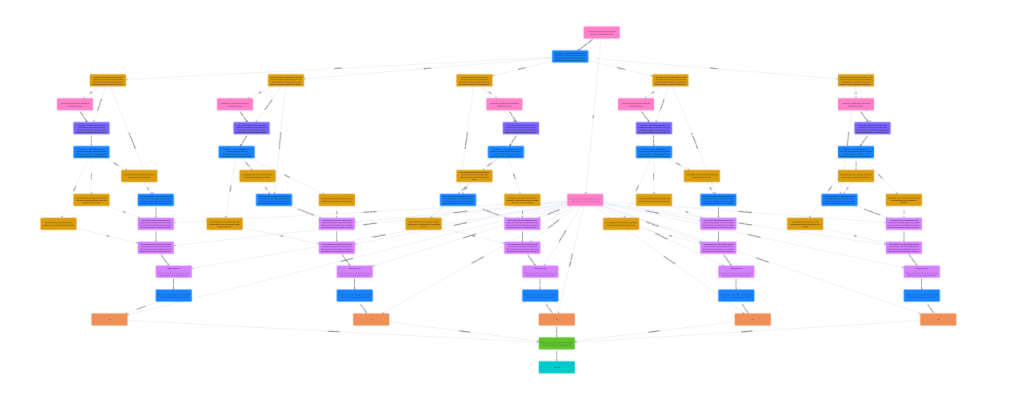
\includegraphics[width=1.0\textwidth]{images/flow_of_thoughts.png}
        \caption{Flow of Thoughts framework using graph visualization, the pink nodes are the nodes from the knowledge graph or definition of the problem, the yellow nodes are generated by the LLM, the purple nodes are refinement of the solution generated by the LLM. In the final layer, the LLM will aggregate the solution and generate the final answer (the cyan node)}
        \label{fig:flow_of_thoughts}
    \end{figure}

    The framework is designed to be a general framework that can be applied to any problem that can be solved by LLMs.

\subsection{Novelty of the solution}

The Flow of Thoughts framework introduces a new approach to processing and extracting relevant information from a large data corpus that might be space for the necessary information to solve the target problem using Self-RAG and a Graph of Thoughts structure, significantly enhancing the efficiency, relevance, and quality of interactions with long-form content. 

This model provides more explainability by recording how LLMs get the final solution from aggregating the partial information gained from Self-RAG. Through its intelligent segmentation, contextual relevance filtering, and ability to compose well-supported answers, this framework can potentially stand out in the landscape of text processing and information retrieval technologies.

\subsection{Efficiency}

Compared with a normal Graph of Thoughts, the framework proposed independent approaches to solve the problem and solve it automatically with self checking for common mistakes and refine the solution along each step. This use generation of LLM more effectively since each path is independent and the LLM can generate more diverse solutions compared to the normal Graph of Thoughts or Tree of Thoughts.

Moreover, the framework intelligently filters irrelevant sections based on the posed question and methods, enabling the model to focus solely on pertinent information. This specificity enhances the accuracy of the responses generated by the LLM and saves costs when dealing with large data corpus.

Compared with a normal Self-RAG Inference, the framework provides more flexibility for the convergence of information for black-boxed models like ChatGPT and Claude. It's easier to migrate to a new model without training the retriever and fine-tuning costs.

\section{Experiment results}

Now we have implemented basic functions for the Flow of Thoughts in revised Graph of Thoughts framework and let the LLM decide whether to use those messages or not when aggregating the final answer.

\subsection{Sorting}

The sorting task is a basic task that can be solved by Graph of Thoughts. we give the LLM a list of random numbers and let it sort them. 

\subsection{Set Intersection}

The set intersection task is a basic task that also can be solved by Graph of Thoughts. We have implemented the basic functions for the Flow of Thoughts with the same functionality as Graph of Thoughts and compare the performance with Graph of Thoughts.

We use the same dataset as the Graph of Thoughts and compare the performance with Graph of Thoughts. However, due to time constraints, we only have the set intersection task results for length 64 and 100 trials using ChatGPT-4o and Claude-3.5-sonnet models.

\subsection{Reading Comprehension}

For the reading comprehension task, we use the RACE dataset \cite{lai2017large} to test the performance of the Flow of Thoughts framework. The dataset contains 28,000+ passages and 100,000+ questions, which is a large dataset for reading comprehension tasks. We use the top 100 passages with longest length to test the performance of the Flow of Thoughts framework. (min passage length 3850, detail of the passages can be found in the appendix)


\section{Analysis}

\section{Limitations and potential future work}

\subsection{Approach generation}
The generated methods may still not be approachable for LLM to execute (Shor’s algorithm to factorize large primes)

Among all the generated methods, most of them are approachable for LLM to execute and will not affect the major voting procedure of the final answer. However, this statement may not hold for more complex problems. The model may need access to external knowledge or API to execute some of the methods. One further improvement is to let the LLM access to external knowledge or API to execute some of the methods as described in ToolLLM \cite{qin2023toolllmfacilitatinglargelanguage}.

\subsection{High expense for graph generation}

During the experiment, we found that the generation of the graph is expensive. The generation of the graph is $O(nm)$ where $n$ is the number of approaches and $m$ is the number of checking steps for each method. (Maybe we can share and check some common mistakes to save costs for improvements) We tried to reuse some of the common mistakes to save costs for improvements. However, the performance is still non-linear especially when the number of mistakes is large.



\medskip
{
\small
\bibliography{references}{}
\bibliographystyle{plain}
}

\section{Appendix}

\subsection{Prompts used in solving the problem}

\subsubsection{Sorting}

For approach generation, we use the following prompt:

Example output:

\subsubsection{Set Intersection}

\subsubsection{Reading Comprehension}

Passages used for reading comprehension test can be found in github repository \url{https://github.com/Trance-0/Flow-of-Thoughts/tree/main/flow-of-thoughts/test/reading_comprehension/RACE_min}

For approach generation, we use the following prompt:

Example output:


\end{document}
